%!TEX TS-program = xelatex
%!TEX encoding = UTF-8 Unicode

\def \papersize {a4paper}
\documentclass[12pt,\papersize]{extarticle}
% extarticle is like article but can handle 8pt, 9pt, 10pt, 11pt, 12pt, 14pt, 17pt, and 20pt text

\def \ititle {Mindreading and Joint Action: Philosophical Tools}
\def \isubtitle {Notes for Lecture 3}
\def \iauthor {Stephen A. Butterfill}
\def \iemail{ButterfillS@ceu.hu}
%for anonymous submisison
%\def \iauthor {}
%\def \iemail{}
%\date{}

\input{$HOME/Documents/submissions/preamble_steve_paper2}

%avoid overhang
\tolerance=5000


\begin{document}

\setlength\footnotesep{1em}

\bibliographystyle{newapa} %apalike

%these two lines are for anonymous submission --- they remove author and date
%but don't forget to remove defs above as well --- otherwise it will be in the metadata
%\author{}
%\date{}


\maketitle
%\tableofcontents
%
%\begin{abstract}
%\noindent
%***
%\ 
%
%\noindent
%\textbf{Keywords:}
%Mindreading, Joint Action, Action, Belief, Intention, Representation, Mental State
%\end{abstract}
%



\section{Question}
This lecture is about a simple question.
\begin{quote}
What could someone represent that would enable her to track, at least within limits, others' perceptions, knowledge states and beliefs including false beliefs? 
\end{quote}
%
One answer is obvious: she might track these things by virtue of representing them as such, that is, by representing perceptions, beliefs, and other propositional attitudes in all the complexity that human adults, in their most reflective moments, grasp.

You might initially doubt that there could be any other answer.
Could abilities to track false beliefs (say) really involve anything other than representing false beliefs?

\section{Slide}
To see the possibility of a positive answer it may help to consider a non-mental analogy.
What could someone represent that would enable her to track, at least within limits, the toxicity of potential food items?
Here the most straightforward answer (she could represent their toxicity) is clearly not the only one.
After all, someone might track toxicity by representing odours or by representing visual features associated with putrefaction, say.
If certain odours reliably indicate toxicity and if you avoid foods which have those odours,
then you are tracking the toxicity of the food.

\section{Slide}
When I say `tracking', all I mean is this.
To \textit{track} the toxicity of a food item is for your thoughts or actions to nonaccidentally depend in some way on how toxic the food item is.

And similarly for belief.

To \textit{track} a subject's belief that $p$ is for your thoughts or actions to nonaccidentally depend in some way on whether this subject believes that $p$.

\section{Slide}
My question, put very roughly, is whether belief has something like an odour.
And my aim in this lecture is to argue that it does.

There is a form of cognition---minimal theory of mind---which does not involve representing mental states as full-blown propositional attitudes but rather involves relying on a simpler model of mental states as relational.
Minimal theory of mind 
is  rich enough to enable systematic success on tasks held to be acid tests for theory of mind cognition including many false belief tasks.
As I'll explain, this may help us to understand what enables those with limited cognitive resources or little conceptual sophistication, such as infants, chimpanzees, scrub-jays and human adults under load, to track, within limits, facts about perceptions and beliefs.

But before I get on to answering the question, I want first to explain how we have arrived at it, how it follows from the discussion of previous lectures.
It’s actually at least as hard to explain why the question matters as it is to answer it.

\section{Slide}
Recall this puzzle from Lecture 1
...

\section{Gap in Notes}

\section{Slide}
A process is \emph{automatic} if whether it occurs is to a significant degree independent of its relevance to the particulars of the subject's motives and aims.

[...]

Against the automaticity of representing belief,
\citet{back:2010_apperly} found that subjects are significantly slower to answer an unexpected question about another's true or false belief compared with matched questions about reality \citep[see also][]{apperly:2006_belief}.
This suggests that, at least in adults, belief tracking is not automatic.
There is also evidence that, even in relatively simple situations, 
using facts about others' beliefs is not automatic \citep{Keysar:2003xu,apperly:2010_limits}.
The case for nonautomaticity is indirectly supported by evidence that tracking perceptions and beliefs---and even merely holding in mind what another believes, where no inference is required---involves a measurable processing cost  \citep{apperly:2008_back,apperly:2010_limits}, consumes attention and working memory in fully competent adults (\citealp{Apperly:2009cc, lin:2010_reflexively, McKinnon:2007rr} experiments 4-5), may require inhibition \citep{bull:2008_role} and makes demands on executive function \citep{apperly:2004_frontal,samson:2005_seeing}.
These findings, taken together, suggest that tracking others' perceptions and beliefs is sometimes not automatic.

The question was whether, in adult humans,  tracking perception and belief is automatic.  
If we assume, further, that either all such processes are automatic or else none are, then the evidence leaves us with a contradiction.


\section{Slide}
I think both puzzles motivate us to ask, 
What is it to represent a belief (or a desire, any other mental state)?
This was the question we asked in the previous lecture.
I suggested that when someone represents a belief, there are two parameters to specify.


\section{Gap in Notes}
[see notes in slides]

\section{Slide}
Second, you have to specify what sort of model they are using of the attitudes.
This is analogous to specifying what sort of model someone is using when they represent mass or force---they might be thinking about these things in terms of the roles they have classical or quantum theories for example, or in some other way.
Last week I tried to suggest there are simpler and more complex models of the attitudes.
I wanted us to focus on decision theory as a model of belief and desire and how they might interact to produce actions because this is such a well-studied model, and one that seems to be realised by a wide range of structures from large organizations to parts of human motor control.
I didn’t mean to suggest that there are stronger reasons for being interested in decision theory, however.

The key thought from last week was just this.
An engineer doesn’t particularly care about the accuracy of the physical models that she uses.
She only cares that they are accurate enough for her purposes.
Further, she often faces a trade-off between accuracy and efficiency.  
Using the most accurate models might demand too much in the way of limited resources.
And so she will trade accuracy for efficiency.
Further, she might made different trade-offs in different projects.
For one project she might use a less accurate model, 
or even just a collection of heuristics;
whereas for another project she might know that it’s worth using a more accurate model.
And, finally, which models she can use might depend on her experience and training.
I want to suggest that it is possible in principle to think of mindreaders as like engineers.
We have more and less accurate models of the attitudes.
For example, decision theory captures something about mental states but not everything: it is an approximation that can be implemented without incurring great costs.
And we might use more and less accurate models on different occasions.


\section{Minimal theory of mind}
\label{sec:minimal}
In this section we begin with someone, call her Lucky, capable  of representing nonintentional behaviour only and ask what more is needed for minimal theory of mind cognition.  We describe Lucky’s progress with a series of principles. The principles are constructed in such a way that it would be coherent to suppose that Lucky has the abilities codified by the first \textit{n} principles only.

The approach is inspired by a tradition of creature construction in philosophy, and in particular by Bennett’s construction in \textit{Linguistic Behaviour} (\citeyear{Bennett:1976rg}).  Of course, where Bennett and others aimed to understand something about what it is for a subject to have desires, beliefs and other mental states, our main aim is to understand what might be involved in tracking and thinking about these things.




\subsection{Second [=first] principle}
Before describing the second principle we need to introduce two concepts.
An agent’s \textit{field} at any given time is a set of objects.  Whether an object falls within the agent’s field is determined by spatial and physical constraints such as proximity and lighting.  The agent’s orientation and posture will also play a role in determining which objects fall into an agent’s field, as will eye direction in some species.  To fall within an agent’s field, there must be no opaque barriers between the agent and the object, unless the object was recently in motion and not behind a barrier.  These constraints ensure that objects which fall into an agent’s field are approximately those the agent can perceive.\footnote{ 	A variety of research in spatial and motor cognition suggests that adult humans (and perhaps others) not only compute other agents’ fields but also spontaneously locate objects within the spatial perspectives of other agents \citep[e.g.][]{en_1700, en_1701}.  }

Let us say that an agent is \textit{encountering} an object if it is in her field.  The notion of encountering defines a relation between an agent and an object.  Within limits, this notion of encountering can do some of the work that the concept of perception does.  Encountering an object is like perceiving one to the extent that both notions involve a relation between agents and objects, both notions have approximately the same extension (someone perceives an object just if she encounters it), and both notions are bound up with action, as we shall explain.  
%This is why representing encounterings and exploiting principles linking encountering to goal-directed action could enable Lucky to track perceptions.

But encountering also differs from perceiving.
If perceptions are representations, then representing perceptions as such plausibly involves representing representations.
Since encounterings are relations not representations (by definition), representing encounterings will  differ from representing perceptions in that only the latter involves representing representations.
And unlike perception, encountering does not involve 
appearances, modalities or the possibility of illusion 
and is not constitutively linked to reasons, knowledge or informational states.

With these concepts in place, we can state the second principle: 
one cannot goal-directedly act on an object unless one has encountered it.  
More carefully,
if an outcome involves a particular object
and the agent has not encountered that object,
then that outcome cannot be a goal of her actions.
As with the other principles, this is plainly not a fact.
What matters is just that, in a limited but useful range of cases, the principles collectively enable lucky to track perceptions and goal-directed actions.

The second principle has many applications.  Someone who is aware of this principle can be motivated to prevent others from encountering her food even when they are not in a position to steal it immediately.  Take scrub-jays.  When choosing where to cache food in the presence of a competitor they prefer far to near, darker to lighter, and occluded to in-view locations \citep[]{en_1451, en_1452}.  These scrub-jays may be trying to hinder future thefts, for these behaviours are not found when caching non-food items \citep[]{en_1419} or when caching in the presence of a partner \citep[][p.\ 514]{Clayton:2007fh, Emery:2007ze}.  Clayton and Emery note that `[s]uch skills suggest visual perspective taking—computing what another can or cannot see' \citep[]{en_1451}. That is to say, they ascribed to scrub jays the concept of seeing.  Another possibility is that scrub-jays compute encountering rather than seeing.  Perhaps scrub-jays take having encountered food to be a condition for performing goal-directed actions targeting that food.  If so they may be trying to minimize the chance that others will encounter their food in order to prevent future theft.  
Of course we  are not claiming that this is the actual explanation of these findings.  
Our question is not about what scrub-jays actually represent but about what someone could represent that would enable her to track perceptions.
Our claim is that the ability to track perceptions in the ways scrub-jays do could involve representing encounterings only.




For another application of the second principle, consider Hare, Call and Tomasello’s finding that chimpanzees reliably adopt strategies which are appropriate given what dominant competitors know about the locations of food \citep[]{en_1545}.  In their `uninformed' condition, a subordinate chimpanzee observed a food item being hidden while a dominant competitor’s view was blocked (see Figure \vref{figure:hare_food_perception}).  In this condition subordinates chose to approach the food significantly more often than in a control condition where the dominant competitor saw the food being hidden.  This indicates that the subordinate chimpanzees were at least indirectly sensitive to facts about what the dominants had perceived.  Several explanations of this finding have already been suggested \citep[]{Call:2008di, en_1551, Suddendorf:2003co}.  A further possibility is that subordinate chimpanzees are aware that the dominant chimpanzee has not encountered the food and take encountering the food to be a condition for the dominant to act with the goal of recovering it.  That would enable them to predict that the subordinate will not be able to retrieve this food in the misinformed condition. 



\begin{figure}
\begin{center}
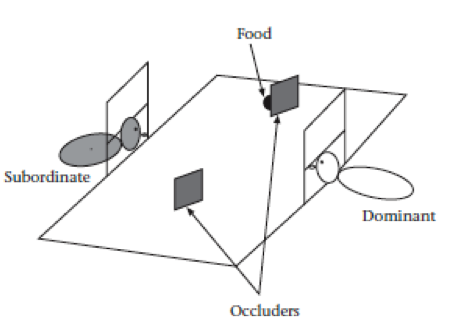
\includegraphics{figure_hare_food_perception.png}
\caption{
	\label{figure:hare_food_perception}
	A subordinate observes as food is placed.  The subordinate can also see the dominant.  There are three conditions: control—the dominant sees food being placed; `uninformed'—the dominant’s view is blocked while the food is placed; and `misinformed'—the dominant sees the food being placed then  has their view blocked while it is moved.
	 \citep[Source:][pp.\ 142, fig. 1]{en_1545}
}
\end{center}
\end{figure}


In short, 
abilities to track others' perceptions  may depend on representing perceptions as such.
But another way to track perceptions would be to represent encounterings and to suppose (as the second principle states) that goal-directed actions involving an object are only possible when the agent has encountered that object.


\subsection{Third principle}

At this point we switch our attention from conditions on the \textit{occurrence} of goal-directed actions to conditions on their \textit{success}. 

Here we need a new notion, \textit{registration}.  Registration is a relation between an individual, an object and a location which will be implicitly defined by principles linking it to encountering and action.  

The first  principle defining registration is that an individual registers an object at a location if and only if she most recently encountered it at that location.  

Registration is like belief in that it has a correctness condition which may not obtain: a registration is correct when the object is in the location.   

The the third principle states that correct registration is a condition of successful action.  More precisely, in order to successfully perform a goal-directed action with a goal that specifies a particular object, the agent must correctly register that object.\footnote{
This principle can be applied in two directions.  In one direction, it licenses Lucky to predict that a competitor who does not have a correct registration of an object will not be successful in performing actions whose goals specify that object.  In the other direction, it allows Lucky, on the basis of observing a successful goal-directed action, to infer that the agent has correctly registered the location of an object.
}

The correctness of someone’s registrations can be manipulated in their absence by moving or destroying objects they have registered.  So with theory of mind cognition partially characterized by the third principle, Lucky can intentionally prevent others from stealing a food item they have already encountered simply by moving it in their absence.

For an application of this principle, consider Hare, Call and Tomasello’s (\citeyear[]{en_1545}) experiment again.  In a further condition, the `misinformed' condition, a subordinate observer watched as a dominant competitor saw food being hidden.  The subordinate continued to watch as the competitor’s view was blocked and the food moved.  In this case the competitor has encountered the food but does not correctly register it.  
Subordinate observers went for the food more often in this condition than in a control condition where the dominant saw the food being moved.  
This cannot be explained in terms of the second principle.  That principle involved taking encountering an object to be a condition on acting on it.  This condition is met: the competitor \textit{has} encountered the food.  To explain why the subordinate observer goes for the food that has been moved, we need to appeal to the third principle—to correct registration as a condition on success.  It is possible that the subordinate observer realized that the dominant competitor last encountered the food in a location other than its current location.  Suppose the observer also understood that correct registration is a condition on successful goal-directed action.  Then the observer could predict that the competitor would not succeed in retrieving the food.  This could explain why  subordinate observers  more often approach the food in the `misinformed' condition than in the control condition.  

\subsection{Fourth principle}

So far Lucky thinks of correct registration as a condition for the success of goal-directed action.  This does not tell her anything about what happens if the condition is not met.  In particular it tells her nothing about how an agent will act when she registers an object incorrectly.  The fourth principle involves a switch from thinking of registration as a success condition to thinking of it as a causal factor.  This principle states that when an agent performs a goal-directed action with a goal that specifies a particular object, the agent will act as if the object were in the location she registers it in.

Now that Lucky understands registration as a factor influencing action it can serve her as a proxy for false belief.  Just as, in a limited but useful range of cases, you can track food sources' toxicities by representing their odours
%, objects’ masses by measuring their weights (within limits) 
and prospective sexual partners’ virtues by representing their plumage, so also you can track beliefs by representing registrations.

Applications of the fourth principle therefore include Onishi and Baillargeon’s (\citeyear[]{en_1092}) false belief task.  Infant subjects are shown an adult observer who is present while a piece of melon is placed in one box.  In the critical condition, the adult observer is then absent while the melon moves to another box.  Comparative looking times indicate that the subjects, who are 14-month-old infants, expect that the adult will reach into the box not containing the melon.\footnote{ 	This finding is supported by a growing body of related research \citep[including][]{en_1666, en_1690, en_1691, en_1208, en_1261}.}  The authors explain this finding by hypothesizing that the infants are ascribing beliefs about the melon’s location to the adults \citep[][p.\ 257]{en_1092}.  Alternatively, the findings could be explained on the hypothesis that they are tracking registration as a cause of action.

\subsection{Extensions and variations}
With the fourth principle we have completed the construction of a minimal theory of mind capable of underwriting success on some false belief tasks.  


\subsection{Extensions and variations}
With the fourth principle we have completed the construction of a minimal theory of mind capable of underwriting success on some false belief tasks.  
This is probably not sufficient to explain infants' or nonhuman animals' abilities to track beliefs and other mental states.
But of course additional principles can be added accommodate further theory of mind abilities.  
We stop here because false belief tasks are often taken to be an acid test for theory of mind.



\section{Limits: how to distinguish minimal from full-blown theory of mind cognition}
\label{sec:limits1}
How could we distinguish minimal from full-blown theory of mind cognition experimentally?  The point of minimal theory of mind is to enable agents to fake it—that is, to act as if they were reasoning about propositional attitudes, within limits.  Where a task goes beyond these limits, we can be sure an agent is not using minimal theory of mind only.

Some limits on minimal theory of mind cognition arise from the fact that the theory makes use of objects and their relations to agents, rather than representations of objects, to predict others’ behaviours.  This means that false beliefs involving quantification or identity cannot be tracked by representing registrations.  To see why not, consider the following inference:
%
\begin{quote}
(1) Mitch believes that Charly is in Baltimore.

(2) Charly is Samantha.

Therefore:

(3) Mitch believes that Samantha is in Baltimore.
\end{quote}
%
On almost any account of belief, this inference is not valid
\citep[][pp.\ 214-5]{frege:1948_sense}.  Its central role in a popular film \citep[]{en_1793} indicates that human adults typically appreciate that this inference is not valid.  Contrast the above inference with the corresponding inference in the case of registration:
%
\begin{quote}
(1$'$) Mitch registers \(<\)Charly, Baltimore\(>\)

(2) Charly is Samantha.

Therefore:

(3$'$) Mitch registers \(<\)Samantha, Baltimore\(>\)
\end{quote}
%
This inference from (1$'$) and (2) to (3$'$) is logically valid.  It is valid because registration is a relation to objects.  We can compare registration with other relations like being left of something.  If Charly is Samantha (whether you know it or not), then anyone who is left of Charly is left of Samantha; similarly for registering Charly’s location. 

This formal difference between belief and registration entails a limit on minimal theory of mind cognition.  Consider Lucky who tracks beliefs by means of representing registrations only and is unable to represent beliefs. Lucky should have no problem predicting actions based on false beliefs about the locations of objects but she should encounter difficulties in predicting actions based on beliefs essentially involving mistakes about identity.  In particular, Lucky should not be able to understand why, when Mitch registers \(<\)Charly, Baltimore\(>\), he continues searching for Samantha.\footnote{ 	This assumes that Lucky herself knows that Charly is Samantha.  To ease exposition we assume throughout that Lucky has no false beliefs involving identity.}  For to register \(<\)Charly, Baltimore\(>\) is the same thing as registering \(<\)Samantha, Baltimore\(>\). And Lucky should be equally at a loss when those she observes someone mistakenly believe that two distinct people are identical.  By contrast, subjects who can represent beliefs as such should have no special problem with false beliefs essentially involving identity.  This is how mistakes about the identities of objects can be used to distinguish minimal from full-blown theory of mind cognition.%
\footnote{ 	
Related points about quantification entail further testable distinctions.  For instance, minimal theory of mind should make it impossible to track beliefs whose contents essentially involve \textit{most} objects having a certain property.  It is beyond the scope of this paper to elaborate on these predictions.
}

How could this be exploited experimentally?  

***Low and Watts (2012) 




\section{Conclusion}

Abilities to track 
perceptions and beliefs are  sometimes but not always  automatic in human adults.   
But representing beliefs and other propositional attitudes as such is associated with demands on working memory, inhibition or attention that are incompatible with automaticity.
This motivated asking what  someone could represent that would enable her to track perceptions, knowledge states and beliefs without meeting these cognitive demands.

Further motivation for asking this question comes from the puzzle from lecture 1.  
It is useful to identify what could represent that would enable her to track, in a limited but useful range of situations, perceptions, knowledge states and beliefs, including false beliefs.  

To answer this question we constructed a minimal theory of mind.  The construction is  rich enough to explain systematic success on tasks held to be acid tests for theory of mind cognition including many false belief tasks.  
%It is also extensible in ways that can explain a range of findings from non-human animals and human infants that are often presented as evidence for full-blown theory of mind cognition.  
Where minimal theory of mind must break down is in cases involving quantification or mistakes about identity (see Section \ref{sec:limits1}).  
Because such cases require full-blown theory of mind, it is possible to distinguish whether an individual’s performance on a particular task involves minimal or full-blown theory of mind cognition. 

The novelty of our constructive approach lies in several features.  It does not rely directly on everyday psychological concepts, whose exact nature is a source of controversy.
Nor does it rely on infants or non-human animals holding theoretical commitment to simplified versions of these concepts (contrast 
	\citealp{en_75};
	\citealp{en_81};
	\citealp{en_2372} and
	\citealp{en_1614}%
).
Importantly, we do not assume that minimal theory of mind develops into full-blown theory of mind in humans.  
It may instead remain distinct, supporting cognitively efficient theory of mind across the lifespan \citep[see][]{Samson:2010jm, en_2397}.  The construction of minimal theory of mind is systematic enough to generate testable predictions distinguishing it from both behavioural stratetgies and full-blown theory of mind cognition (see Sections \ref{sec:limits1} and \ref{sec:limits2}).  
Our construction makes detailed sense of the notion that there are degrees of theory of mind cognition.  
(This is a virtue because while is widely recognised that degrees of theory of mind cognition are needed \citep[e.g.][]{en_610, en_1415}, there have been few detailed attempts to make systematic sense of this possibility.)
It also pushes much further than earlier work the boundaries of what can be achieved without full-blown theory of mind cognition; in particular, it explains how systematic success on a range of false belief tasks (but not those which essentially involve identity or quantification) is possible without representing beliefs or other propositional attitudes as such. Minimal theory of mind may be what enables those with limited cognitive resources or little conceptual sophistication, such as infants, chimpanzees, scrub-jays and human adults under load,  to track others'  perceptions, knowledge states and beliefs. 








\small
\bibliography{$HOME/endnote/phd_biblio}

\end{document}